\chapter{Introduction to binaries}
Binary analysis can be carried out with two different techniques:
\begin{itemize} 
    \item Static Analysis: 
        \subitem \textcolor{green}{The entire binary can be potentially analysed in one go}; 
        \subitem\textcolor{green}{No need for an architecture capable of running the binary};
        \subitem \textcolor{red}{No knowledge of the runtime states};
    \item Dynamic Analysis: \subitem \textcolor{green}{Often simpler};
        \subitem \textcolor{green}{Possibility to observe a particular execution};
        \subitem \textcolor{red}{Chance to miss interestingparts of the code}; 
        \subitem \textcolor{red}{Potentially dangerous if analysisng malware}; 
        \end{itemize} 
It can present several challenges as: 
\begin{itemize} 
    \item it is in a low level language - i.e. Assembly - that can present itself in different flavours 
    (AT\&T, Intel, non x86 platforms); 
    \item There might be no symbols (e.g.  stripped binaries);
    \item Code and data are mixed together; 
    \item Impossible to remove/add instructions without "bricking" the program. 
\end{itemize} 
\section{Execution} 
Unless one is programming the bare metal, programs are generally executed on an Operating System (OS hereafter) which 
is an \textbf{abstract machine}.  A running profram is a process, which has its own resources and can use a subset of 
the ISA (implemented on the actual CPU or emulates), an abstract model of a CPU and the API of the OS (e.g. syscall).
\subsection{Emulation, Virtualisation, Containers}
As computers became more accessible to people the idea of simply time sharing the machine became unfeasible; system had
to be made reduntant and fault tolerant whilst being able to be shared across the entire userbase. Having multiple
systems is beneficial for:
\begin{itemize} 
    \item \textbf{Isolation} Systems must be isolated for stability reasons in such a way that programs do not interfere
        with each other for stability (i.e. buggy programs shall not cause disruption to other processes);
    \item  \textbf{Performance} Placing an application on it's own system allows it to have exclusive access to the
        system's resources. User level segregation does not effectively isolate applications as scheduling priority,
        memory demand, network and FS I/O can generate interference between programs.  
\end{itemize} 
However having multiple systems is not always the most fruitful and effective solution and in the 60's IBM started
working on the first \textit{virtual machines} where it was crucial to be able to time-share expensive main frames.
A VM is a fully isolated copy of the underlying hardware that enable applications to run as they were on "bare metal".
\subsubsection{Virtual Machine Monitor}
The VMM is the software component that hosts the virtual machines; the VMM is
generally called \textit{host} and the VM's are called \textit{guests}.  It's duties are, among the others, the
provision of virtulised CPU, virtualised resources such as I/O devices, storage, memory and isolation between VM's.
\subsubsection{Internet Services Virtualisation} In order to face the ever more demanding Internet applications a new
kind of system was adopted: the multi-tier system architecture. THis common way of building Internet applications
entails the separation of the web and database server and easily enables load-balancing and clustering. The system has 
the advantage of being easier to manage and extremely fault tolerant, but this requires the additional cost of additional 
hardware purchases and management.
In this scenario the system virtualisation provides the advantages of componitisation without the need for additional 
hardware (and exacerbated by Zipf's law\footnote{The frequency of an event is proportional to $x^{-\alpha}$ where $x$ 
is the rank of the event in comparison to other events}). Studies have found that the internet services behave according
to a Zipfian distribution, i.e. if we observe the web caches we see that only a few web services are always active and 
used the most of the others just lay dormant; thus isolation is no longer a worthy option unless services are
consolidated to a single machine and virtualisation provides the best benefit for the cost as it avoids the waste of
computing power and reduces the maintenance costs.
\subsubsection{Requirements for VM's} 
In 1974 Popek and Goldberg defined what they believed where the formal requirements for a virtualisable computer
architecture: \textit{"For any computer a virtual machine monitor can be constructed if the set of instructions is a
subset of the privileged instructions"}; the most essential requirement a computer architecture must have in order to
be virtualisable is that privileged instructions must launch a trap and render control to the VMM so it can decide
whether the instruction can be executed or not. The three essential characteristics of VM's are:
\begin{enumerate}
    \item Any program run under the VMM should exhibit an effect identical with that demonstrated if the program had
        run on the original machine (with the exception of the timing effects related to the virtualisation overhead);
    \item A statistically dominant subset of the virtual processor's instructions are directly executed by the real
        processor - i.e. the virtual machine occasionally relinquishes the real processor to the virtual processor; 
    \item The VMM is in complete control of system resources and the virtual machine does not have direct access to the
        system's real resources.
\end{enumerate}
\subsection{Full System Virtualisation}
Full sytem virtualisation provides avirtual replica of the system's hardware so that the OS's and software may run on
the VM exactly as it would on "bare metal".
\subsubsection{370-XA Virtualisation}
The VM/370 is a VMM that was first delivered in the VMF/370 and ran the 370-XA, an architecture designed to maximise 
the virtualisation performance. The platform provided \textit{"assists"} in the architecture to boost the
virtualisation performance of certain repetitive operations. The VMM had to simulate the instruction beforehand to 
ensure safety; the assist development allowed the execution of the simulated instructions on the hardware. Other 
assists supplanted the frequently executed instructions that still required VMM intervention and were enabled by
setting them in \textit{interpretive execution} mode. Assists included VMA, ECPS, STB and many others (IBM developed
more than 100 in total).
\subsubsection{IA-32} 
It was the most dominating architecture (now supplanted by x64) but it was never meant to be virtualised although that
would have had enormous benefits; the reason behind this resides in the fact that there is a limited subset of
instructions that does not need higher privilege to be run and cripple a machine. This is not a problem in systems 
with single OS, but it becomes difficult to manage when multiple OS's are running at once. Furthermore the huge amount 
of different devices and drivers for the IA-32 made virtualisation a big deal. However IA-32 has been finally
virtualised according to the following:
\begin{enumerate} 
    \item Non-sensitive,
        non-privileged instructions may be run directly on the processor;
    \item Sensitive, Privileged instructions trap - i.e. the processor sends an interrupt and the VMM instercepts it 
        for proper management of the instruction
    \item Sensitive, but not privileged instructions are detected and the VMM ensures they never get executed as they 
        cannot be handled with a trap.
\end{enumerate}
\subsubsection{IA-64} 
It presents more or less the same drawbacks of the
IA-32, but it provides an important feature as it allows to run VM's in a higher ring of the VMM and traps from the
higher rings can be intercepted by lower rings.
\subsubsection{Drawbacks of full system virtualisation} 
The advantage of full system virtualisation is that OS's and programs can run unmodified and completely oblivious of the
environment in which they are actually running. However there are drawbacks related to the fact that IA-32 and IA-64
were not created to be virtualised and thus a lot of effort must be put into efficiently virtualising hardware and
memory management. When an application demands for a memory page the system translates the virtual address to a
physiscal one thanks to page table. Unused pages can be written to disk when inactive or when more memory is required.
The VMM must intercept all of the memory calls and translate VM space into the system's real space using another pag table,
retrieve the memory and return it to the VM.
\subsection{Paravirtualisation}
Paravirtualisation tries to mitigate the performance hit by modifying the OS so that tasks are performed by the VMM
directly and not by the CPU. There are several commecrcial and open solutions that can efficiently carry out
paravirtualisation like:
\begin{itemize} 
    \item Xen Project;
    \item Citrix Xen Server;
    \item Denali;
    \item VMWare Sphere;
\end{itemize} 
The VMM provides the VM's with a software interface that is similar yet not entirely identical to the underlying
hardware. Paravirtualisation provides specifically defined hooks by which it tries to minimise the number of
operations that must be carried out in the virtual environment. The guest OS shall be modified for the
paravirtualisation API, although this requirement is less strict nowadays as more and more paravirtualsation
enabled components can be found under the GPL and other free licenses.
\subsection{Other virtualisation techniques}
There are other virtualisation techniques like: 
\begin{itemize} 
    \item Emulation: replication of a specific architecture that enables a machine to behave like another;
    \item Containerisation: OS-level virtualisation that allows for the presence of isolated user-space instances 
        called containers.  
\end{itemize} 
\section{Binaries} 
Executables are created in compliance with a specific ABI that depends on the architecture. The ABI establishes: 
\begin{itemize} 
    \item The executable and object file formats;
    \item fundamental types (size alignment for int, long and other primitives);
    \item How data types are laid out in memory;
    \item Function and system call conventions;
    \item How programs are started up (initialisation, dynamic linking, etc.) 
\end{itemize}
\subsection{Executable and Linkable Format} It is a flexible format that can be used for:
\begin{itemize}
    \item executables; 
    \item dynamic libraries (*.so);
    \item object files (also called relocatable files).
\end{itemize}
The ELF format is a sequence of headers, segments and sections containing the necessary information and data for the 
execution and linkage of the executable.
\subsubsection{File Header}
The file header is located at the beginning of the file and is used to locate the other parts.
\begin{lstlisting}[style=ansic, caption={File Header}, label=ehdr] 
typedef struct
{ 
    unsigned char e_ident;
    Elf64_Half e_type;
    Elf64_Half e_machine;
    Elf64_Word e_version;
    Elf64_Addr e_entry;
    Elf64_Off  e_phoff;
    Elf64_Off  e_shoff;
    Elf64_Word e_flags;
    Elf64_Half e_ehsize;
    Elf64_Half e_phentsize;
    Elf64_Half e_phnum;
    Elf64_Half e_shentsize;
    Elf64_Half e_shnum;
    Elf64_Half e_shstrndx;
} Elf64_Ehdr; 
\end{lstlisting}
where: 
\begin{itemize} 
    \item {\ttfamily e\_ident} is an array of bytes that identifies the file as an ELF and provides info about the data representation of the object file structures. The bytes of the identifier are:
    \subitem {\ttfamily e\_ident[EI\_MAG0], e\_ident[EI\_MAG1], e\_ident[EI\_MAG2], e\_ident[EI\_MAG3]} contain the so called magic number '0x7fELF';
    \subitem {\ttfamily e\_ident[EI\_CLASS]} identifies the class of the ELF (32bit or 64bit);
    \subitem {\ttfamily e\_ident[EI\_DATA]} specifies the encoding of the object file data structures (little or big endian);
    \subitem {\ttfamily e\_ident[EI\_VERSION]} identifies the version of the object file format and is     presently set to EV\_CURRENT which has value 1;
    \subitem {\ttfamily e\_ident[EI\_OSABI]} identifies the OS and ABI version for which the object file is prepared. Some fields in other ELF structures have flags that can be interpreted based on the value of this field;
    \subitem {\ttfamily e\_ident[EI\_ABIVERSION]} Identifies te version of the ABI fdor which the binary is prepared. The interpretation of this field depends on the value of the {\ttfamily e\-ident[EI\_OSABI]};
    \item {\ttfamily e\_type} Identifies the object file type and its values can be:\newline
    \begin{center}
        \begin{tabular}{|c|c|c|} \hline \textbf{Name} & \textbf{Value} & \textbf{Purpose} \\ 
            \hline {\ttfamily ET\_NONE} & 0x0000 & No file type \\
            \hline {\ttfamily ET\_REL} & 0x0001 & Relocatable file type \\
            \hline {\ttfamily ET\_EXEC} & 0x0002 & Executabler \\
            \hline {\ttfamily ET\_DYN} & 0x0003 & Shared Object \\
            \hline {\ttfamily ET\_CORE} & 0x0004 & Core File \\
            \hline {\ttfamily ET\_LOOS} & 0xFE00 & Environment specific use \\
            \hline {\ttfamily ET\_HIOS} & 0xFEFF & Environment specific use\\
            \hline {\ttfamily ET\_LOPROC} & 0xFF00 & Processor specific use\\
            \hline {\ttfamily ET\_HIPROC} & 0xFFFF & Processor specific use\\
            \hline 
        \end{tabular} 
    \end{center} 
    \item {\ttfamily e\_machine} identifies the architecture;
    \item {\ttfamily e\_version} identifies the version of the current file format;
    \item {\ttfamily e\_entry} contains the virtual address of the entry point;
    \item {\ttfamily e\_phoff} contains the file offset in bytes of the program header table;
    \item {\ttfamily e\_shoff} contains the offset in bytes of the section header table;
    \item {\ttfamily e\_flags} contains processor specific flags;
    \item {\ttfamily e\_ehsize} contains the size in bytes of the ELF header;
    \item {\ttfamily e\_phentsize} contains the size in bytes of a progam header entry;
    \item {\ttfamily e\_phnum} contains the number pf entries in the program header table;
    \item {\ttfamily e\_shentsize} contains the size in bytes of a section headeer table entry;
    \item {\ttfamily e\_shnum} contains the number of entries in the section header table;
    \item {\ttfamily e\_shstrndx} section header table index of the string table.
\end{itemize}
\subsubsection{Sections}
The code and data in an ELF binary are logically divided into contiguous nonoverlapping chunks called sections; their structure is not predetrmined and varies depending on the content.  Sections contain all the information in an ELF file, with the exception of the file header and can be identified by their index into the section header table.  Strictly speaking the organisation into sections is intended to be convenient at linking; hence not all of the sections are actually needed while setting up a process and the virtual memory (e.g.  symbols and relocation sections do not contain info needed during execution). As sections are only there for the linker the presence of the section header   table is not mandatory (and the {\ttfamily e\_shoff} is set to 0 in this case).
\paragraph{Section Indices}
Section indices 0, 0xFF00-0xFFFF are reserved for special purposes as per the following: 
\begin{center}
    \begin{tabular}{|c|c|p{6cm}|} 
        \hline \textbf{Name} 	& \textbf{Value} 	& \textbf{Description}\\
        \hline SHN\_UNDEF & 0 & Used to mark undefined or meaningless section reference\\
        \hline SHN\_LOPROC & 0xFF00 & Processor-specific use\\
        \hline SHN\_HIPROC & 0XFF1F & Processor-specific use\\
        \hline SHN\_LOOS & 0xFF20 & Environment-specific use\\
        \hline SHN\_HIOS & 0xFF3F & Environment-specific use\\
        \hline SHN\_ABS & 0xFFF1 & Indicates that the reference is an absolute value\\
        \hline SHN\_COMMON & 0xFFF2 & Indicates a symbol that has been declared as a common block (tentative declaration in C)\\
        \hline
     \end{tabular}
 \end{center}
\textcolor{red}{The first entry in the section header table (at index 0) \textbf{MUST} contain all zeroes}. \paragraph{Section Header Entries} The structure of a section header is as per the following \begin{lstlisting}[style=ansic, caption={Section Header}, label=shdr]
typedef  struct
{
    Elf64_Word sh_name;
    Elf64_Word sh_type; 
    Elf64_Xword sh_flags; 
    Elf64_Addr sh_addr; 
    Elf64_Off sh_offset;
    Elf64_Xword sh_size;
    Elf64_Word sh_link;
    Elf64_Word sh_info;
    Elf64_Xword sh_addralign;
    Elf64_Xword sh_entsize;
} Elf64_Shdr;
\end{lstlisting} where:
\begin{itemize}
\item {\ttfamily sh\_name} contains the offset, in bytes, to the section name relatively to the start of the section name string table;
\item {\ttfamily sh\_type} identifies the section type detailed as follows:
\begin{center}
                                \begin{tabular}{|c|c|p{6cm}|} \hline \textbf{Name} & \textbf{Value} & \textbf{Meaning} \\ \hline
                {\ttfamily SHT\_NULL} & 0 & Marks an unused section header \\ \hline {\ttfamily SHT\_PROGBITS} &
                1 & Contains program data such as machine instructions and constants \\ \hline {\ttfamily
                SHT\_SYMTAB} & 2 & Contains the static linking symbol table \\ \hline {\ttfamily SHT\_STRTAB} &
                3 & Contains a string table \\ \hline {\ttfamily SHT\_RELA} & 4 & Contains "Rela" type
                relocation entries \\ \hline {\ttfamily SHT\_HASH} & 5 & Contains a symbol hash table \\ \hline
                {\ttfamily SHT\_DYNAMIC} & 6 & Contains dynamic linking tables\\ \hline {\ttfamily SHT\_NOTE} &
                7 & Contains note information\\ \hline {\ttfamily SHT\_NOBITS} & 8 & Contains uninitialised
                space; does not occupy any space in the file\\ \hline {\ttfamily SHT\_REL} & 9 & Contains "Rel"
                type relocation entries\\ \hline {\ttfamily SHT\_SHLIB} & 10 & Reserved\\ \hline {\ttfamily
                SHT\_DYNSYM} & 11 & Contains a dynamic loader symbol table\\ \hline {\ttfamily SHT\_LOOS} &
                0x6000 0000 & Environment-specific use\\ \hline {\ttfamily SHT\_HIOS} & 0x6FFF FFFF &
                Environment-specific use \\ \hline {\ttfamily SHT\_LOPROC} & 0x7000 0000 & Processor-specific
            use\\ \hline {\ttfamily SHT\_HIPROC} & 0x7FFF FFFF & Processor-specific use\\ \hline \end{tabular}
        \end{center} \item {\ttfamily sh\_flags} identifies the attributes of the section name as listed:
            \begin{center} \begin{tabular}{|c|c|p{6cm}|} \hline \textbf{Name} & \textbf{Value} &
                \textbf{Meaning} \\ \hline {\ttfamily SHF\_WRITE} & 0x1 & Contains writeable data\\ \hline
                {\ttfamily SHF\_ALLOC} & 0x2 & Section allocated in memory image of a program\\ \hline
                {\ttfamily SHF\_EXECINSTR} & 0x4 & Contains executable instructions\\ \hline {\ttfamily
            SHF\_MASKOS} & 0x0F00 0000 & Environment-specific use\\ \hline {\ttfamily SHF\_MASKPROC} & 0xF000
            0000 & Processor-specific use\\ \hline \end{tabular} \end{center} \item {\ttfamily sh\_addr}
                contains the virtual address of the beginning of the section in memory. If the section is not
            allocated in memory this shall be 0; \item {\ttfamily sh\_offset} contains the offset of the section
            in bytes from the beginning of the file; \item {\ttfamily sh\_size} contains the size of the section
            (unless it's a {\ttfamily SHT\_NOBITS}); \item {\ttfamily sh\_link} contains the index of an
                associated section.  This field is used for several purposes as detailed in the following:
                \begin{center} \begin{tabular}{|c|c|} \hline \textbf{Type} & \textbf{Associated Section} \\
                    \hline {\ttfamily SHT\_DYNAMIC} & String table used by entries in this section\\ \hline
                {\ttfamily SHT\_HASH} & Symbol table in which the hash table applies\\ \hline {\ttfamily
                SHT\_REL/RELA} & Symbol table referenced by the relocations\\ \hline {\ttfamily
                SHT\_SYMTAB/DYNSYM} & String table used in entries used in these sections\\ \hline \end{tabular}
    \end{center} \item {\ttfamily sh\_info} contains extra info about the section as explained below:
        \begin{center} \begin{tabular}{|c|c|} \hline \textbf{Type} & \textbf{Info} \\ \hline {\ttfamily
            SHT\_REL/RELA} & Index of the section which the relocation applies to\\ \hline {\ttfamily
        SHT\_SYMTAB/DYNSYM} & Index of the first non-local symbol (i.e. number of local symbols)\\ \hline
        \end{tabular} \end{center} \item {\ttfamily sh\_addralign} contains the required alignment of the
        section and must be a power of 2; \item {\ttfamily sh\_entsize} contains the size in bytes, of each
entry, for sections that contain fixed-size entries (zero otherwise).  \end{itemize} The standard sections for
Code/Data and other object file are reported in tables \ref{codedata} and \ref{objfile}.  \begin{table}[!htbp]
    \begin{center} \begin{tabular}{|c|c|c|c|} \hline \textbf{Name} & \textbf{Type} & \textbf{Flags} &
        \textbf{Use}\\ \hline {\ttfamily .bss} & {\ttfamily SHT\_NOBITS} & {\ttfamily SHF\_ALLOC/WRITE} &
        Uninitialised data\\ \hline {\ttfamily .data} & {\ttfamily SHT\_PROGBITS} & {\ttfamily SHF\_ALLOC/WRITE}
        & Initialised data\\ \hline {\ttfamily .interp} & {\ttfamily SHT\_PROGBITS} & {\ttfamily SHF\_ALLOC} &
        Program interpreter path name\\ \hline {\ttfamily .rodata} & {\ttfamily SHT\_PROGBITS} & {\ttfamily
        SHF\_ALLOC} & Read only data (const and literals)\\ \hline {\ttfamily .text} & {\ttfamily SHT\_PROGBITS}
        & {\ttfamily SHF\_ALLOC/EXECINSTR} & Executable code\\ \hline \end{tabular} \caption{Code and Data
Standard Sections} \label{codedata} \end{center} \end{table} \begin{table}[!htbp] \begin{center}
    \begin{tabular}{|c|c|c|c|} \hline \textbf{Name} & \textbf{Type} & \textbf{Flags} & \textbf{Use}\\ \hline
        {\ttfamily .comment} & {\ttfamily SHT\_PROGBITS} & {\ttfamily None} & Version Control Info\\ \hline
        {\ttfamily .dynamic} & {\ttfamily SHT\_DYNAMIC} & {\ttfamily SHF\_ALLOC/WRITE} & Dynamic Linking
        Tables\\ \hline {\ttfamily .dynstr} & {\ttfamily SHT\_STRTABS} & {\ttfamily SHF\_ALLOC} & String table
        for the {\ttfamily .dynamic} segment\\ \hline {\ttfamily .dynsym} & {\ttfamily SHT\_DYNSYM} & {\ttfamily
        SHF\_ALLOC} & Read only data (const and literals)\\ \hline {\ttfamily .got} & {\ttfamily SHT\_PROGBITS}
        & {\ttfamily machine dependent} & Global Offset Table\\ \hline {\ttfamily .hash} & {\ttfamily SHT\_HASH}
        & {\ttfamily SHT\_ALLOC} & Symbol Hash Table\\ \hline {\ttfamily .note} & {\ttfamily SHT\_NOTE} &
        {\ttfamily none} & Note Section\\ \hline {\ttfamily .plt} & {\ttfamily SHT\_PROGBITS} & {\ttfamily
        machine dependent} & Procedure Linkage Table\\ \hline {\ttfamily .rel[\textit{name}]} & {\ttfamily
        SHT\_REL} & {\ttfamily SHT\_ALLOC} & Relocations for section [\textit{name}]\\ \hline {\ttfamily
        .rela[\textit{name}]} & {\ttfamily SHT\_RELA} & {\ttfamily SHT\_ALLOC} & As Above \\ \hline {\ttfamily
        .shstrtab} & {\ttfamily SHT\_STRTAB} & {\ttfamily None} & Section Name String Table\\ \hline {\ttfamily
        .strtab} & {\ttfamily SHT\_STRTAB} & {\ttfamily None} & String Table\\ \hline {\ttfamily .symtab} &
    {\ttfamily SHT\_SYMTAB} & {\ttfamily SHT\_ALLOC} & Linker Symbol Table\\ \hline \end{tabular} \caption{Other
Object Files Standard Sections} \label{objfile} \end{center} \end{table} \subsection{String Table} Contains the
strings used for section and symbol names. It is an array of null terminated strings. Section header table
entries, and symbol table entries refer to strings in a string table with an index relative to the beginning of
the string table.  \textcolor{red}{The first byte of the table must be null so that the index 0 always refers to
a non-existent name.} \subsection{Symbol Table} The first symbol table entry is reserved and must be all zeroes
({\ttfamily STN\_UNDEF} is useed as a reference to this entry).  The structure of a symbol table entry is
\begin{lstlisting}[style=ansic, caption={Symbol Table Entry}, label=shdr]
typedef  struct
{
    Elf64_Word      sh_name;
    unsigned char 	st_info;
    unsigned char 	st_other;
    Elf64_Half 		st_shndx;
    Elf64_Addr      st_value;
    Elf64_Xword     st_size;
} Elf64_Sym;
\end{lstlisting} where: 
\begin{itemize} 
\item {\ttfamily st\_name} contains the offset in
bytes to the symbol name from the beginning of the string table;
\item {\ttfamily st\_info} contains the symbol type and its binding attributes - i.e. the scope. The binding attributes are contained in the high-order 4 bits of the eight bit byte and the symbol type is contained in the lower order 4 bits. The availble bindings and types are reported in tables \ref{bindings} and \ref{types}. 
\begin{table}[!htbp]
 \begin{center}
     \begin{tabular}{|c|c|c|c|} 
         \hline \textbf{Name} & \textbf{Value} & \textbf{Description}\\
         \hline {\ttfamily STB\_LOCAL} & 0 & Not visible out of the object files\\
         \hline {\ttfamily STB\_GLOBAL} & 1 & Visible to all object files\\
         \hline {\ttfamily STB\_WEAK} & 2 & Global but with lower precedence\\
         \hline {\ttfamily STB\_LOOS} & 10 & Env specific use\\
         \hline {\ttfamily STB\_HIOS} & 12 & Env specific use\\
         \hline {\ttfamily STB\_LOPROC} & 13 & Processor specific use\\
         \hline {\ttfamily STB\_HIPROC} & 15 & Processor specific use\\
         \hline
     \end{tabular}
 \caption{Symbol Bindings}
 \label{bindings}
\end{center}
\end{table}
\begin{table}[!htbp]
\begin{center}
    \begin{tabular}{|c|c|c|c|}
        \hline \textbf{Name} & \textbf{Value} & \textbf{Description}\\
        \hline {\ttfamily STT\_NOTYPE} & 0 & No type\\
        \hline {\ttfamily STT\_OBJECT} & 1 & Data Object\\
        \hline {\ttfamily STT\_FUNC} & 2 & Function entry point\\
        \hline {\ttfamily STT\_SECTION} & 3 & Symbol is associated with a section\\
        \hline {\ttfamily STT\_FILE} & 4 & Source file associated with the object file\\
        \hline {\ttfamily STT\_LOOS} & 10 & Env specific use\\
        \hline {\ttfamily STT\_HIOS} & 12 & Env specific use\\
        \hline {\ttfamily STT\_LOPROC} & 13 & Processor specific use\\
        \hline {\ttfamily STT\_HIPROC} & 15 & Processor specific use\\
        \hline 
    \end{tabular}
\caption{Symbol Types}
\label{types}
\end{center} 
\end{table}
\item {\ttfamily st\_other} is reserved for future use and must be 0; \item {\ttfamily st\_shndx}
    contains the index of the section the index is defined into. For undefined symbols it is {\ttfamily
SHN\_UNDEF}, for absolute symbols it is {\ttfamily SHN\_ABS} and for common ones is {\ttfamily
SHN\_COMMON}; \item {\ttfamily st\_value} contains the value of the symbol. it may be aboslute or
relocatable address. In relocatable files this field contains the alignment constraint for common
symbols and a section relative offset for defined relocatable symbol. In executables and standard object
files this contains a virtual address for the defined relocatable symbol.  \item {\ttfamily st\_size} contains
the size associated with the symbol. If a symbol does not have an associated size this field contains 0.
\end{itemize}
\subsection{Relocations} These sections contain information used by the linker to perform relocations; essentially these are tables with each entry detailing a particular address at whic the relocation must be performed along with the instructions to resolve the value that needs to be plugged at that value. Of course static relocations are resolved at compile time and only dynamic will remain. These sections can be {\ttfamily .rel.*} or {\ttfamily .rela.*} and their type defines the symbol resolution method.
\paragraph{.rel.*} The {\ttfamily .rel.*} sections contain the addend part of the relocation from the original part and are smaller than {\ttfamily .rela.*}. The underlying data structure is reported in \ref{rel}.
\begin{lstlisting}[style=ansic, caption={.rel.* entries}, label=rel]
typedef  struct
{
    Elf64_Addr r_offset; // Address of reference
    Elf64_Xword r_info;  // Symbol index and type of relocation
} Elf64_Rel;
\end{lstlisting}
\paragraph{.rela.*} This is larger than the former and provides an explicit field for the full addend.
\begin{lstlisting}[style=ansic, caption={.rel.* entries}, label=rel]
typedef  struct
{
    Elf64_Addr r_offset;   // Address of reference
    Elf64_Xword r_info;    // Symbol index and type of relocation
    Elf64_Sxword r_addend; // Constant part of the expression
} Elf64_Rela;
\end{lstlisting} where:
\begin{itemize}
    \item {\ttfamily r\_offset} indicates the location at which the relocation must be applied.  For a relocatable file this is the offset, in btes, from the beginning of the section to the beginning of the storage unit being relocated. For an executable or shared object, this is the virtual address of the storage unit being relocated.
    \item {\ttfamily r\_info} contains both a symbol table index and a relocation type. The symbol table index identifies the symbol which value should be used in the relocation.  The type instead qualifies the method used for the relocation; these can vary wildly in the real world, but the most important are {\ttfamily R\_X86\_64\_GLOB\_DAT} and {\ttfamily R\_X86\_64\_JUMP\_SLO}.
        \subitem The first one is used to compute the address of a data symbol and plug it in the correct offset into the {\ttfamily .got} section.
        \subitem The latter is called jump slot and they have their offset in the {\ttfamily .got.plt} (the stubs in the PLT use them to compute the jump target as an offset from the {\ttfamily rip} register).  They can be identified by application of the macro in \ref{elf64relmacros}.
        \begin{lstlisting}[style=ansic,caption={Macros},label=elf64relmacros]
#define ELF64_R_SYM(i)((i) >> 32)
#define ELF64_R_SYM(i)((i) & 0xffffffff)
#define ELF64_R_INFO(s, t)(((s) << 32) + ((t) & 0xffffffff))
       \end{lstlisting}
    \item {\ttfamily r\_addend} specifies a constant addend used to compute the value to be stored in the relocated field.  \end{itemize}
\subsection{Program Header Table} The program header table provides the segment view as opposed to the section perspective detailed above and has a different purpose indeed. In fact sections are exclusively relevant to the static linker, while segments are used by the dynamic linker when loading an ELF into a process for execution to locate the relevant code and data and decide what to load in virtual memory. A single segment may contain multiple sections. The underlying data structure can be found in listing \ref{elf64phdr}
\begin{lstlisting}[style=ansic, caption={Program Header}, label=elf64phdr]
typedef  struct 
{
    Elf64_Word 	p_type;    // Segment type
    Elf64_Word 	p_flags;   // Segment attributes Elf64_Off 	p_offset;  // Constant part of the expression
    Elf64_Addr 	p_vaddr;   // Virtual address in memory 
    Elf64_Addr  p_paddr;   // Reserved
    Elf64_Xword p_filesz;  // Size of the segment in the file
    Elf64_Xword p_memsz;   // Size of the segment in memory
    Elf64_Xword p_align;   // Alignment of segment
} Elf64_Rela; 
\end{lstlisting} 
where:
\begin{itemize}
    \item {\ttfamily p\_type} indicates the type of the segment and can have the following values:
    \begin{table}[!htbp]
        \begin{center}
            \begin{tabular}{|c|c|c|}
                \hline \textbf{Name} & \textbf{Value} &  \textbf{Description}\\
                \hline {\ttfamily PT\_NULL} & 0 & Unused entry\\
                \hline {\ttfamily PT\_LOAD} & 1 & Loadable segment\\
                \hline {\ttfamily PT\_DYNAMIC} & 2 & Dynamic linking tables\\
                \hline {\ttfamily PT\_INTERP} & 3 & Program interpreter path\\
                \hline {\ttfamily PT\_NOTE} & 4 & Note sections\\
                \hline {\ttfamily PT\_SHLIB} & 5 & Reserved\\
                \hline {\ttfamily PT\_PHDR} & 6 & Program header table\\
                \hline {\ttfamily PT\_LOOS} & 0x60000000 & Environment specific use\\
                \hline {\ttfamily PT\_HIOS} & 0x6FFFFFFF & Environment specific use\\
                \hline {\ttfamily PT\_LOPROC} & 0x70000000 & Processor specific use\\
                \hline {\ttfamily PT\_HIPROC} & 0x7FFFFFFF & Processor specific use\\
                \hline 
            \end{tabular}
        \caption{Segment types}
        \label{segtypes}
        \end{center}
    \end{table}
    The fields {\ttfamily PT\_LOAD}, {\ttfamily PT\_DYNAMIC} and {\ttfamily PT\_INTERP} are particularly important.  {\ttfamily PT\_LOAD} segments are intended to be loaded into memory when setting up the process. The size of the chunk at the address which it must be loaded at are described in the rest of the program header.  {\ttfamily PT\_INTERP} segments contains the {\ttfamily .interp} section which provides the name of the interpreter that is to be used to load the binary.  {\ttfamily PT\_DYNAMIC} contains the {\ttfamily .dynamic} section which tells the interpreter how to parse and prepare the binary for execution \item {\ttfamily p\_flags} contains the segment attributes. The top eight bits are reserved for processor specific use and the others are reserved for environment specific use. The possible attributes can assume the values: 
    \begin{table}[!htbp]
        \begin{center}
            \begin{tabular}{|c|c|c|}
                \hline \textbf{Name} & \textbf{Value} & \textbf{Description}\\
                \hline {\ttfamily PF\_X} & 0x1 & Execute permission\\
                \hline {\ttfamily PF\_W} & 0x2 & Write permission\\
                \hline {\ttfamily PF\_R} & 0x4 & Read permission\\
                \hline {\ttfamily PF\_MASKOS} & 3 & Environment reserved\\
                \hline {\ttfamily PF\_MASKPROC} & 4 & Precessor reserved\\
                \hline
            \end{tabular}
            \caption{Segment types}
            \label{segtypes}
        \end{center}
    \end{table}
    \item {\ttfamily p\_offset} contains the offset of the segment, in bytes, from the beginning of the file;
    \item {\ttfamily p\_vaddr} contains the virtual address of the segment in memory (for loadable segments this must be equal to the offset);
    \item {\ttfamily p\_paddr} is reserved for the physical address, but in modern OS's is  generally set to 0 (most of today's systems use virtual addresses);
    \item {\ttfamily p\_filesz} and {\ttfamily p\_memsz} contain respectively the size of the file image and the memory image of the segment. These are different as some sections only indicate the need to allocate some bytes but don't actually occupy these bytes in the bynary file (e.g. {\ttfamily .bss} contains zero initialised data and since all data in this section are zero there is no need to actually include them in the binary, but all of its bytes are allocate when it is loaded into memory). Hence it is impossible to have {\ttfamily p\_memsz} bigger than {\ttfamily p\_filesz} and when this happens the loader adds extra bytes initialised to zero.
    \item {\ttfamily p\_align} specifies the alignment constraints for the segment and must be a powero of two. The {\ttfamily p\_offset} and {\ttfamily p\_vaddr} must be congruent modulo the alignment.
\end{itemize}
\subsection{Notes}
Sections of type {\ttfamily SHT\_NOTE} and {\ttfamily PT\_NOTE} are used by compilers and other tools to mark an object file with special info that has a special meaning for a particular toolset. These sections and segments contain any number of note entries, each of which is an 8-byte word. A note contains:
\begin{itemize}
    \item {\ttfamily namesz} and {\ttfamily name}. The first identifies the length of a name in bytes. The latter contains a null terminated string, padded to 8-byte alignment.  
    \item {\ttfamily descsz} and {\ttfamily desc}. The first identifies the length of the note descripto whilst the second stores the content of the note padded to 8-byte alignment as necessary.
    \item {\ttfamily type} contains a number that determines, along with the oroginator's name, the interpretation of the note contents.
\end{itemize}
\subsection{Dynamic table}
Dynamically bound object files will have a {\ttfamily PT\_DYNAMIC} program header entry that refers to a segment contaaining the {\ttfamily .dynamic} sextion. The content of the section is an array of {\ttfamily Elf64\_Dyn} structures as per the listing below:
\begin{lstlisting}[style=ansic, caption={Dynamic Table Structure}, label=elf64dyn]
typedef struct {
    Elf64_Sxword d_tag;
    union { Elf64_Xword d_val; Elf64_Addr  d_ptr; } 
    d_un;
} Elf64_Dyn;
\end{lstlisting} 
where:
\begin{itemize}
    \item {\ttfamily d\_tag} identifies the type of dynamic table entry. The type determiines the interpretation to be given to the union {\ttfamily d\_un}. The processor-independent dynamic table entry types are
    \begin{table}[!htbp]
        \begin{center}
            \begin{tabular}{|c|c|c|p{10cm}|}
                \hline \textbf{Name} & \textbf{Value} & \textbf{d\_un} & \textbf{Description}\\
                \hline {\ttfamily DT\_NULL} & 0 & ignored & Marks the end of the dynamic array\\
                \hline {\ttfamily DT\_NEEDED} & 1 & {\ttfamily d\_val} & The string table offset of a needed library\\
                \hline {\ttfamily DT\_PLTRELSZ} & 2 & {\ttfamily d\_val} & Total size, in bytes, of the relocation entries associated with the PLT\\
                \hline {\ttfamily DT\_PLTGOT} & 3 & {\ttfamily d\_ptr} & Address associated with the PLT (the specific meaning is processor dependent)\\
                \hline {\ttfamily DT\_HASH} & 4 & {\ttfamily d\_ptr} & Address of the symbol hash table\\
                \hline {\ttfamily DT\_STRTAB} & 5 & {\ttfamily d\_ptr} & Address of the dynamic string table\\
                \hline {\ttfamily DT\_SYMTAB} & 6 & {\ttfamily d\_ptr} & Address of the dynamic symbol table\\
                \hline {\ttfamily DT\_RELA} & 7 & {\ttfamily d\_ptr} & Address of the relocation table with {\ttfamily Elf64\_Rela} entries\\
                \hline {\ttfamily DT\_RELASZ} & 8 & {\ttfamily d\_val} & Total size, in bytes of the {\ttfamily DT\_RELA} table\\
                \hline {\ttfamily DT\_RELAENT} & 9 & {\ttfamily d\_ptr} & Size, in bytes, of the relocation entry\\ \hline {\ttfamily DT\_STRSZ} & 10 & {\ttfamily d\_val} & Total size, in bytes, of the string table\\ \hline {\ttfamily DT\_SYMENT} & 11 & {\ttfamily d\_val} & Size, in bytes, of each symbol table entry\\ \hline {\ttfamily DT\_INIT} & 12 & {\ttfamily d\_ptr} & Address of the initialisation function\\
                \hline {\ttfamily DT\_FINI} & 13 & {\ttfamily d\_ptr} & Address of the termination function\\
                \hline {\ttfamily DT\_SONAME} & 14 & {\ttfamily d\_val} & String table offset of this shared object\\
                \hline {\ttfamily DT\_RPATH} & 15 & {\ttfamily d\_val} & String table offset of a shared library search path\\
                \hline {\ttfamily DT\_SYMBOLIC} & 16 & {\ttfamily ignored} & The presence of this dynamic table entry modifies the symbol resolution algorithm for references within the library. These are resolved befre the dynamic linker searches the usual search path\\
                \hline {\ttfamily DT\_REL} & 17 & {\ttfamily d\_ptr} & Address of the relocation table with {\ttfamily Elf64\_Rel} entries\\
                \hline {\ttfamily DT\_RELSZ} & 18 & {\ttfamily d\_val} & Size in bytes of the {\ttfamily DT\_REL} table\\
                \hline {\ttfamily DT\_RELENT} & 19 & {\ttfamily d\_val} & Size in bytes of the {\ttfamily DT\_REL} relocation entry\\
                \hline {\ttfamily DT\_PLTREL} & 20 & {\ttfamily d\_val} & Type of the relocation entry for the procedure linkage table. The {\ttfamily d\_val} contains either {\ttfamily DT\_REL} or {\ttfamily DT\_RELA}\\
                \hline {\ttfamily DT\_DEBUG} & 21 & {\ttfamily d\_ptr} & Reserved for debugger use\\
                \hline {\ttfamily DT\_TEXTREL} & 22 & {\ttfamily ignored} & The presence of this dynamic table entry signals that the relocation table contains relocation for non-writable segment\\
                \hline {\ttfamily DT\_JMPREL} & 23 & {\ttfamily d\_ptr} & Address of the relocations associated with the {\ttfamily PLT}\\
                \hline {\ttfamily DT\_BIND\_NOW} & 24 & {\ttfamily ignored} & The presence of this dynamic table entry signals that the dynamic loader should process all relocations before transferring control to the program\\
                \hline {\ttfamily DT\_INIT\_ARRAY} & 25 & {\ttfamily d\_ptr} & Pointer to array of pointers to the initialisation functions\\
                \hline {\ttfamily DT\_FINI\_ARRAY} & 26 & {\ttfamily d\_ptr} & Pointer to array of pointers to the termination functions\\
                \hline {\ttfamily DT\_INIT\_ARRAYSZ} & 27 & {\ttfamily d\_ptr} & Size in bytes of the array of initialisation functions\\
                \hline {\ttfamily DT\_FINI\_ARRAYSZ} & 28 & {\ttfamily d\_ptr} & Size in bytes of the array of termination functions\\
                \hline \end{tabular} \caption{Dynamic Table Entries}
            \end{center}
        \end{table}
    \item {\ttfamily d\_val} union member used to represent integer values;
    \item {\ttfamily d\_ptr} union member used to represent link-time virtual addresses that must be relocated to math the actual address at which the object file is loaded. The relocations must be done implicitly and tthere are no dynamic relocations for these items
\end{itemize} 
\subsection{Hash Table} 
The access to the dynamic table is efficiently guaranteed by the use of a hash table that is part of the loaded program segment (typically in the {\ttfamily .hash} section) and is pointed to by the {\ttfamily DT\_HASH} entry in the dynamic table. The hash table is an array of {\ttfamily Elf64\_Word} objects, organised as:
\begin{itemize}
    \item {\ttfamily nbucket}
    \item {\ttfamily nchain}
    \item {\ttfamily bucket[0]...bucket[nbucket - 1]}
    \item {\ttfamily chain[0]...chain[nchain - 1]}
\end{itemize}
The {\ttfamily bucket} array forms the hash table itself. The number of entries in the hash table is given by the first word {\ttfamily nbucket}. The entries in the {\ttfamily chain} reflect the symbol table. Entries of the symbol table are organised in hash chains, one per bucket. The hash function is listed below.
\begin{lstlisting}[style=ansic, caption={Program Header}, label=hashtab]
unsigned long elf64_hash(const unsigned char *name) {
    unsigned long h = 0, g;
    while (*name) {
         h = (h << 4) + *name++;
         if (g = h & 0xF0000000)
            h ^= g >> 24;
        h &= 0x0FFFFFFF; 
        }
    return h;
    } 
\end{lstlisting}
\section{x86/x64}
The x86 is the most widely adopted processor architecture.  Started in 1978 with the 8086 and 8088; the processor had segmentation and supported $2^{20} = 1MB$.  The 286 was issued in 1982; it had protected mode using segment registers as a selector with a maximum supported address space of $2^{24} = 16MB$. The game changer arrived in 1985 with the 386; it was the first 32-bit processor using virtual 8086 mode with support for an address space of $2^{32} = 4GB$ and paging with 4k pages. The 486 (x87), released in 1989, had an FPU. During the end of the 90's/beginning of the 2000 several revolutions happened: \begin{itemize} \item[1993] Pentium (4k and 4M pages); \item[1995-99] P6 family with support for SIMD instructions and vector (MMX and SSE mainly used for multimedia); \item[2000-2007] Pentium 4 and Xeon families, enhanced SIMD (SSE2 and 3), hyperthreading and VT. This family sets a milestone as it sees the introduction of the modern IA64 \end{itemize} And now we come to 2008 with the release of the contemporary Intel Core i3, i5, i7 family with SSE4.2 and second generation VT.
\subsection{Modes of operation} 
The operation modes, also called processor modes, CPU states or privilege level wok basically like gates in the execution of certain instructions. The purpose is to place restrictions on the type and scope of operations that can be performed by certain processes. Memory translation starts every time the CPU executes an instruction that refers to a memory address. The origin of this technique dates back to the 8086 that had 16-bit registers and its instructions used mostly 8 or 16 bit operands allowing the code to work with $2^{16}$ bytes (64K); yet CPU designers wanted to use more memory without expanding the size of the registers. This gave birth to the \underline{segment registers} which are a mean to tell the CPU which 64K long segment had to be used and the effective offset from the beginning of the segment itself.
\subsubsection{16bit}
This is the operation mode of the 8086 and 8088 which are identical from a programming standpoint. They only support 1MB of memory and operate in \underline{real mode} which is unsafe as every program can access the entire memory including memory of other processes and programs. Memory segments cannot be larger than 64K. The 80286 introduced the 16bit protected mode and increased the available memory to 16MB.
\paragraph{Real Address Mode}
In real mode memory is limited to $2^{20}$ bytes (i.e. 1MB) with addresses ranging from 00000 to FFFFF. These require a 20 bit number which of course does not work with the 16 bit limit of the 8086 registers. Intel solved the problem by using two 16-bit values instead of one for addressing:
\begin{enumerate}
    \item \textbf{The Selector} that provides the beginning of the memory segment;
    \item \textbf{The Offset} that is used to calculate the address from the beeginning of the segment.
\end{enumerate}
The address can be calculated according to the formula:
\begin{equation} 
    address = 16 \cdot selector + offset
\end{equation}
Real address mode has disadvantages:
\begin{itemize} 
    \item A single selector can only reference 64K of memory and must be updated if the code is larger than this upper bound;
    \item Each byte in memory does not have a unique segmented address, but multiple offsets from different selectors and comparison might be tricky.
\end{itemize}
\paragraph{16bit Protected Mode}
In 286 protected mode, selector values are interpreted completely differently in real mode. The selector is an index into the LDT/GDT and virtual addresses are used in lieu of physical ones. The entries in the descriptor table contain the info relevant to their respective segment: 
\begin{enumerate}
    \item Presence in memory of the segment; 
    \item Access permissions; 
    \item Location in memory.
\end{enumerate} 
\begin{figure} 
    \begin{center}
        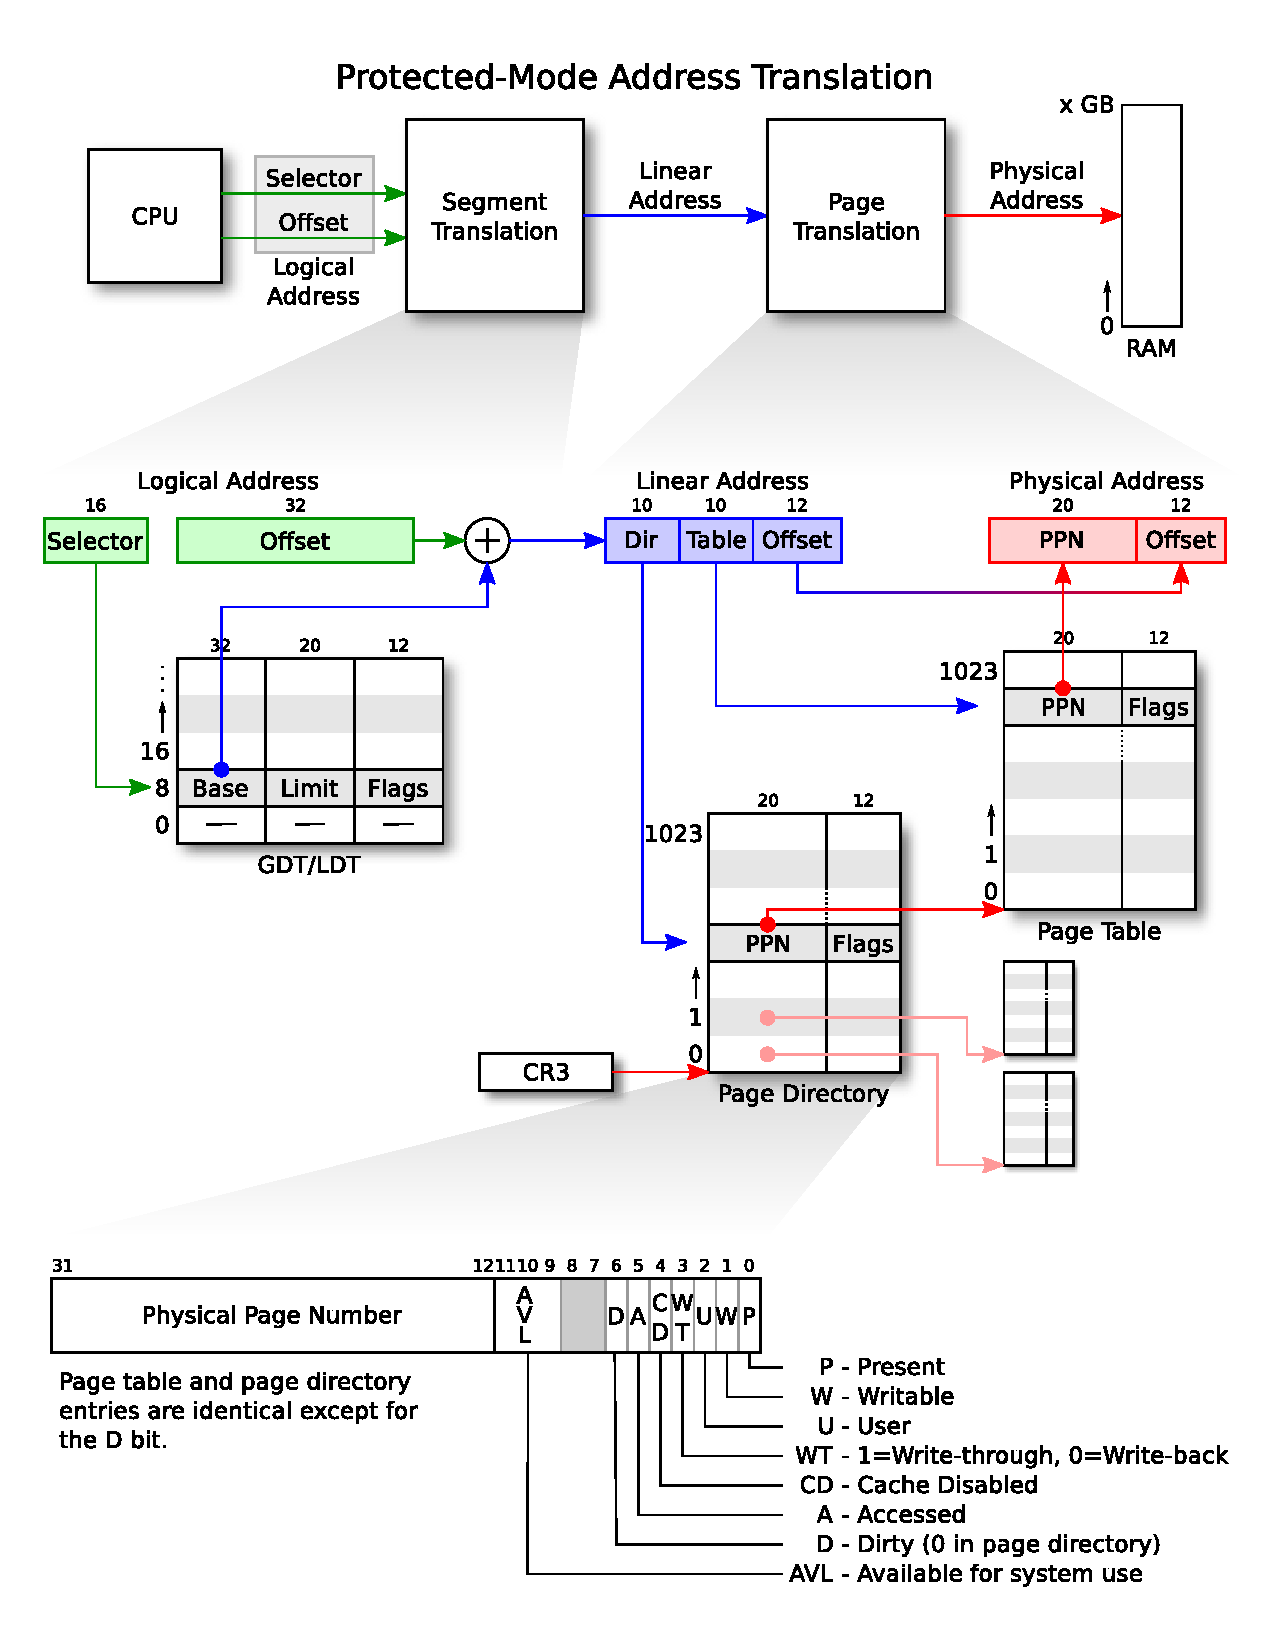
\includegraphics[scale=0.5]{./pics/x86_translation.pdf}
        \caption{Memory Translation}
        \label{memtrans}
    \end{center} 
\end{figure}
\paragraph{Registers} The 8086 had four general purpose registers: AX, BX, CX and DX; each of them can be split into two 8bits - i.e. *H and *L - containing the higher and lower halves of the registers respectively; trivially changing the value of an entire register changes the values of its halves and vice versa. The SI and DI registers can be used very much like their general purpose counterparts, but they cannot be decomposed. The BP and SP are respectively the base and stack pointers. The segment registers are:
\begin{itemize}
    \item[CS] Code Segment;
    \item[DS] Data Segment;
    \item[SS] Stack Segment;
    \item[ES] Extra Segment used as a temporary register.
\end{itemize}
The IP is the instruction pointer and holds the value of the next nstruction to be executed. The FLAGS instead is a collection of bits that contains information related to the result of the last executed instruction.  \subsubsection{32bit} 
The processor boots up in \underline{real-address mode} the 8086 mode) for compatibility. After that it reaches the \underline{32bit protected mode} where execution is carried out according to the privileges established for the relevant execution ring. There is another mode which is the system management mode intended for use by firmware only.  Applications run with a paged 32-bit flat address space having a maximum size of 4GB (as well as 4GB segments).  \paragraph{32bit Protected Mode} The CPU produces a logical address made of a 16bit Selector and the Offset; these are given to the GDT that returns the Base and the Limit of the LDT along with relevant flags. These are combined into the linear address which contains the Page Directory, the Page Table and the Offset. By knowing the page directory and the page table we can find the PPN and with the offset we finally find the address in memory where data and instructions stand.  Modern OS's use paging only to provide a 32/64 bit virtual flat address space.  32bit address space is divided in segments like the 16bit memory, but segments are divided into \textit{pages} which can be loaded separately. \paragraph{Registers} The registers are extended to 32 bits from 16 (hence the use of the E prefix in the name of the registers); they still are general purpose registers although their legacy definition was: 
\begin{itemize}
    \item[EAX] Accumulator; 
    \item[EBX] Data Pointer; \item[ECX] Counter; \item[EDX] I/O Pointer; \item[ESI] Source Pointer for strings;
    \item[EDI] Destination Pointer.
\end{itemize}
The other registers instead still maintain specific roles:
\begin{itemize}
    \item[EIP] Instruction Pointer;
    \item[ESP] Stack Pointer;
    \item[EBP] Base Pointer;
    \item[EFLAGS] like FLAGS.
\end{itemize}
The only registers which are not extended are the segment registers;(ncluding the FS and GS new temporary segments).
\subsubsection{64bit} The 64bit CPUs runs in IA32e, with two submodes:
\begin{enumerate}
    \item \textbf{Compatibility Mode} similar to the 32bit protected mode and permits legacy 32 and 16 bit applications
            to run without being recompiled.  Allows access to $2^{36} = 64GB$ of physical memory using Physical Address Extensions;
    \item \textbf{64 bit Mode} allows to run 64 bit applications, extending general and SIMD registers from 8 to 16.
\end{enumerate}
\paragraph{Registers}
Registers are extended again and they gain the prefix R* with similar scope, but with the following rules: \begin{enumerate}
    \item 64bit operands produce 64bit results;
    \item 32bit operands produce 32bits results with 0 extension of the upper part of the register;
    \item \textcolor{red}{Word and half word operands do not change the upper part of the register.}
\end{enumerate}
\subsection{Operands}
Machine code instructions have a varying number and type of operands; however single instructions will have a fixed number of operands. They can be:
\begin{itemize}
    \item an immediate listed into the instruction itself (hence in the code segment);
    \item a register;
    \item a memory location (which might be hardcoded into the instruction or computed by means of the values in the registers);
    \item implied when thy are not explicitly shown;
    \item an I/O port.
\end{itemize}
\subsection{Instruction Format}
They are bytes strings from one to fiften bytes consisting of the following:
\begin{itemize} 
    \item Optional Prefixes used to override segment/operant sizes and so on;
    \item ModR/M specifies whether the instruction accesses memory or registers respectively;
    \item Immediates which are typically 32 bits in size (when 64bits are necessary they are sign extended).
\end{itemize}

\section{Execution}
This section outlines the detail of the execution of a binary from data representation to function and system calls.

\subsection{Data Representation}
In binary analysis, for x86, data are normally represented in \textit{words} which are 32 bit wide objects; this concept
is weakly used for x86\_64.
\begin{table}[htbp]
    \begin{center}
    \begin{tabular}[|c|c|]
    \begin{figure}
        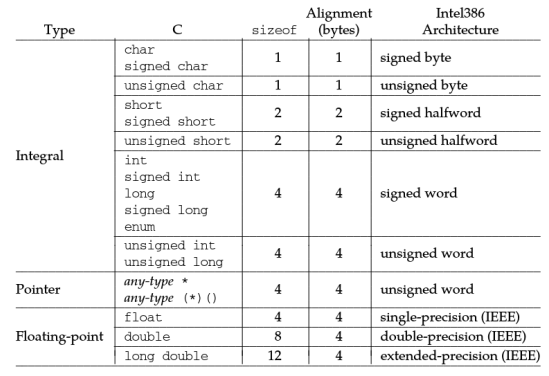
\includegraphics[scale=0.4]{./pics/i386_data.png}
        \caption{32bit data representation}
        \label{32bit_word}
    \end{figure}
        &
    \begin{figure}
        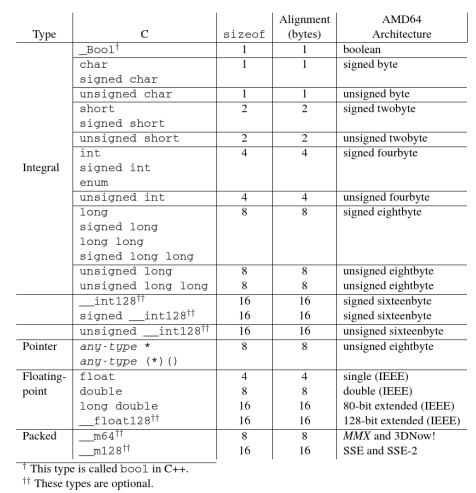
\includegraphics[scale=0.4]{./pics/amd64_data.png}
        \caption{64bit data representation}
        \label{amd64_data}
    \end{figure}
    \end{tabular}
    \end{center}
\end{table}
